%%%%% Kapitola 4 - Návrh uživatelského rozhraní
%%%%% ------------------------------------------------------------
\chapter{Návrh uživatelského rozhraní}
\label{ch:navrh-uzivatelskeho-rozhrani}
Ve světě digitálních produktů a jejich designu jsou uživatelské rozhraní, z anglického \foreign{\acf{ui}}, a uživatelský zážitek, z anglického \foreign{\acf{ux}}, dva pojmy, které se často zaměňují, ačkoli se jedná o velmi odlišné aspekty procesu vývoje produktu.
Tato kapitola si klade za cíl představit koncepty \ac{ui} a \ac{ux}, prozkoumat jejich vzájemný vztah a zabývat se specifiky návrhu \ac{ui} pro aplikaci pro prodej vstupenek s rezervací míst.

\textbf{\ac{ui}} se vztahuje k vizuálním prvkům produktu, se kterými uživatel interaguje – tedy tlačítkům, textu, ikonografii, formulářům a všem vizuálním prvkům, které umožňují uživateli interagovat s produktem.
V kontextu aplikace pro prodej vstupenek s rezervací míst se \ac{ui} vztahuje například k interaktivnímu plánu sedaček, výběru vstupenek, tlačítku pro přechod k dokončení objednávky nebo nákupnímu košíku.

\textbf{\ac{ux}} je na druhou stranu celkový zážitek uživatele při interakci s produktem.
Je ovlivněn snadností použití, hodnotou, kterou uživatel z produktu získává, a emocemi, které jsou při interakci vyvolány.
\ac{ux} bere v potaz celou cestu uživatele, od okamžiku, kdy uživatel do aplikace vstoupí, až po okamžik, kdy dokončí nákup.

Významným aspektem \ac{ux} je uživatelská cesta, z anglického \foreign{User Journey}, která popisuje cestu uživatele při interakci s produktem.
Uživatelská cesta se skládá z jednotlivých kroků, které uživatel musí absolvovat, aby dosáhl svého cíle.

Souhra \ac{ui} a \ac{ux} je v procesu návrhu produktu klíčová.
Dobře navržené \ac{ui} usnadňuje \ac{ux}.
Například intuitivně navržený plán sedadel (\ac{ui}) může proces výběru sedadla zpříjemnit a zjednodušit (\ac{ux}).

Následující sekce této kapitoly prozkoumají základní principy návrhu \ac{ui} a možná použití Maslowovy hierarchie, za účelem návrhu rozhraní více zaměřeného na uživatele.
Dále budou uvedeny a porovnány různé nástroje, které jsou k dispozici pro návrh \ac{ui} a důvody rozhodnutí pro konkrétní nástroj.
Následně budou analyzovány specifikace prototypu z kapitoly~\ref{ch:specifikace} z hlediska \ac{ui}/\ac{ux} se zaměřením na tzv.\ uživatelské příběhy, které tvoří základ \ac{ux} designu.

Závěr této kapitoly bude věnován návrhu interaktivního plánu sedaček, který je klíčovým \ac{ui} prvkem vyvýjeného prototypu aplikace.

%%% Sekce - Principy návrhu uživatelského rozhraní
%%% --------------------------------------------------------------
\section{Principy návrhu uživatelkého rozhraní}
\label{sec:navrh-principy}
Návrh uživatelského rozhraní je poměrně rozsáhlá disciplína, která se zaměřuje na vizuální a interaktivní aspekty produktu.
Při návrhu \ac{ui} je důležité dodržovat určité principy, které zajišťují optimální uživatelskou zkušenost.
Tato sekce shrnuje některé základní principy návrhu \ac{ui} a posuzuje jejich implikace v kontextu aplikace pro prodej vstupenek s rezervací míst.

\textbf{Konzistence}: Tento princip prosazuje zachování jednotnosti napříč všemi prvky \ac{ui}.
Konzistence se projevuje v použití podobných prvků, akcí a designu napříč celým rozhraním.
Například pokud určitá barva značí interaktivní prvek na plánu sedadel, stejná barva by měla být použita i pro značení interaktivních prvků jinde v rámci aplikace.
Tímto se zvyšuje předvídatelnost, což uživatelům usnadňuje orientaci a navigaci v rozhraní.

\textbf{Uživatel v kontrole}: Základním principem návrhu \ac{ui} je umožnit uživateli cítit se vždy v kontrole nad produktem.
Toho lze dosáhnout návrhem transparentního a intuitivního systému, ve kterém uživatel vždy ví, kde se nachází a jak postupovat.
V kontextu aplikace pro prodej vstupenek to může znamenat poskytnutí jasného a zřejmého způsobu, jak uživatelé mohou přejít k výběru sedadla, přidání do košíku a dokončení objednávky.

\textbf{Zpětná vazba}: Zpětná vazba je klíčovým aspektem každé interakce, protože potvrzuje nebo informuje  uživatele o vykonaných akcích.
Vizuální indikátory, jako je zvýraznění vybraného sedadla nebo potvrzovací zpráva při přidání vstupenky do košíku, poskytují uživateli okamžitou zpětnou vazbu.
Tím se snižuje nejistota a zvyšuje se důvěra uživatele v rozhraní.

\textbf{Jednoduchost}: Návrh \ac{ui} by měl směřovat k jednoduchosti.
Čím méně úsilí musí uživatel vynaložit na pochopení rozhraní, tím lepší bude celková uživatelská zkušenost.
Čisté, jednoduché rozhraní s jasným zaměřením na funkčnost snižuje kognitivní zátěž a zvyšuje použitelnost.

\textbf{Prevence a řešení chyb}: Chyby jsou nevyhnutelné v jakékoli interakci, ale dobře navržené \ac{ui} může zabránit většině uživatelských chyb nebo zjednodušit jejich řešení.
To může znamenat například zakázání tlačítka \textit{Pokračovat} dokud není vybráno sedadlo nebo zobrazení jasných a užitečných chybových zpráv, když něco selže.

\textbf{Afordance a signifikance}: \foreign{Afordance} se vztahuje k vlastnosti objektu, která naznačuje, jak se má používat.
\foreign{Signifikance} jsou vizuálními nápovědami k témto \foreign{afordancím}.
Například sedadlo na plánu sedadel může být navrženo tak, aby naznačovalo, že na něj lze kliknout (\foreign{afordance}), a změna kurzoru při najetí na sedadlo (\foreign{signifikance}) může tuto zprávu posílit.

Pochopení a aplikace těchto základních principů návrhu \ac{ui} je klíčové pro vytvoření intuitivního a uživatelsky přívětivého rozhraní.
Tyto principy řídí rozhodnutí v rámci návrhu a pomáhají návrhu \ac{ui} s celkovým cílem poskytnout uživatelům bezproblémový zážitek z rezervace vstupenek.
Další sekce se zabývá tím, jak lze hierarchii Maslowa aplikovat pro další zlepšení uživatelsky orientovaného návrhu.

%%% Sekce - Aplikovaná psychologie na návrh uživatelských rozhraní
%%% --------------------------------------------------------------
\section{Aplikovaná psychologie na UI/UX}
\label{sec:navrh-psychologie}

\epigraph{\textit{``Some people say, "Give the customers what they want." But that's not my approach. Our job is to figure out what they're going to want before they do.''}}{-- Steve Jobs}

Proces návrhu uživatelského rozhraní se netýká pouze estetiky nebo funkcionality v izolaci.
Ve skutečnosti, k vytvoření rozhraní, které skutečně rezonuje s uživateli, si lze vypůjčit koncept z psychologie - Maslowovu hierarchii potřeb.
Tato hierarchie, obvykle vizualizovaná jako pyramidová struktura, ilustruje cestu jednotlivce k seberealizaci a naplnění, začínající od základních fyziologických potřeb až po složitější emoční a psychologické potřeby.

\textit{Maslowova hierarchie potřeb} je teorie psychologa Abrahama Maslowa, která se snaží vysvětlit, co motivuje lidi.
Maslow tvrdil, že lidé mají potřeby, které se snaží uspokojit, ale některé z nich jsou naléhavější než jiné.
Když jsou tyto potřeby uspokojeny, lidé se mohou cítit šťastnější, ale když nejsou, lidé mohou být frustrovaní a nespokojení.\cite{maslow}
Maslow rozdělil lidské potřeby do pěti základních úrovní, které jsou znázorněny na obrázku~\ref{fig:maslow} níže.

\begin{figure}[H]
    \centering
    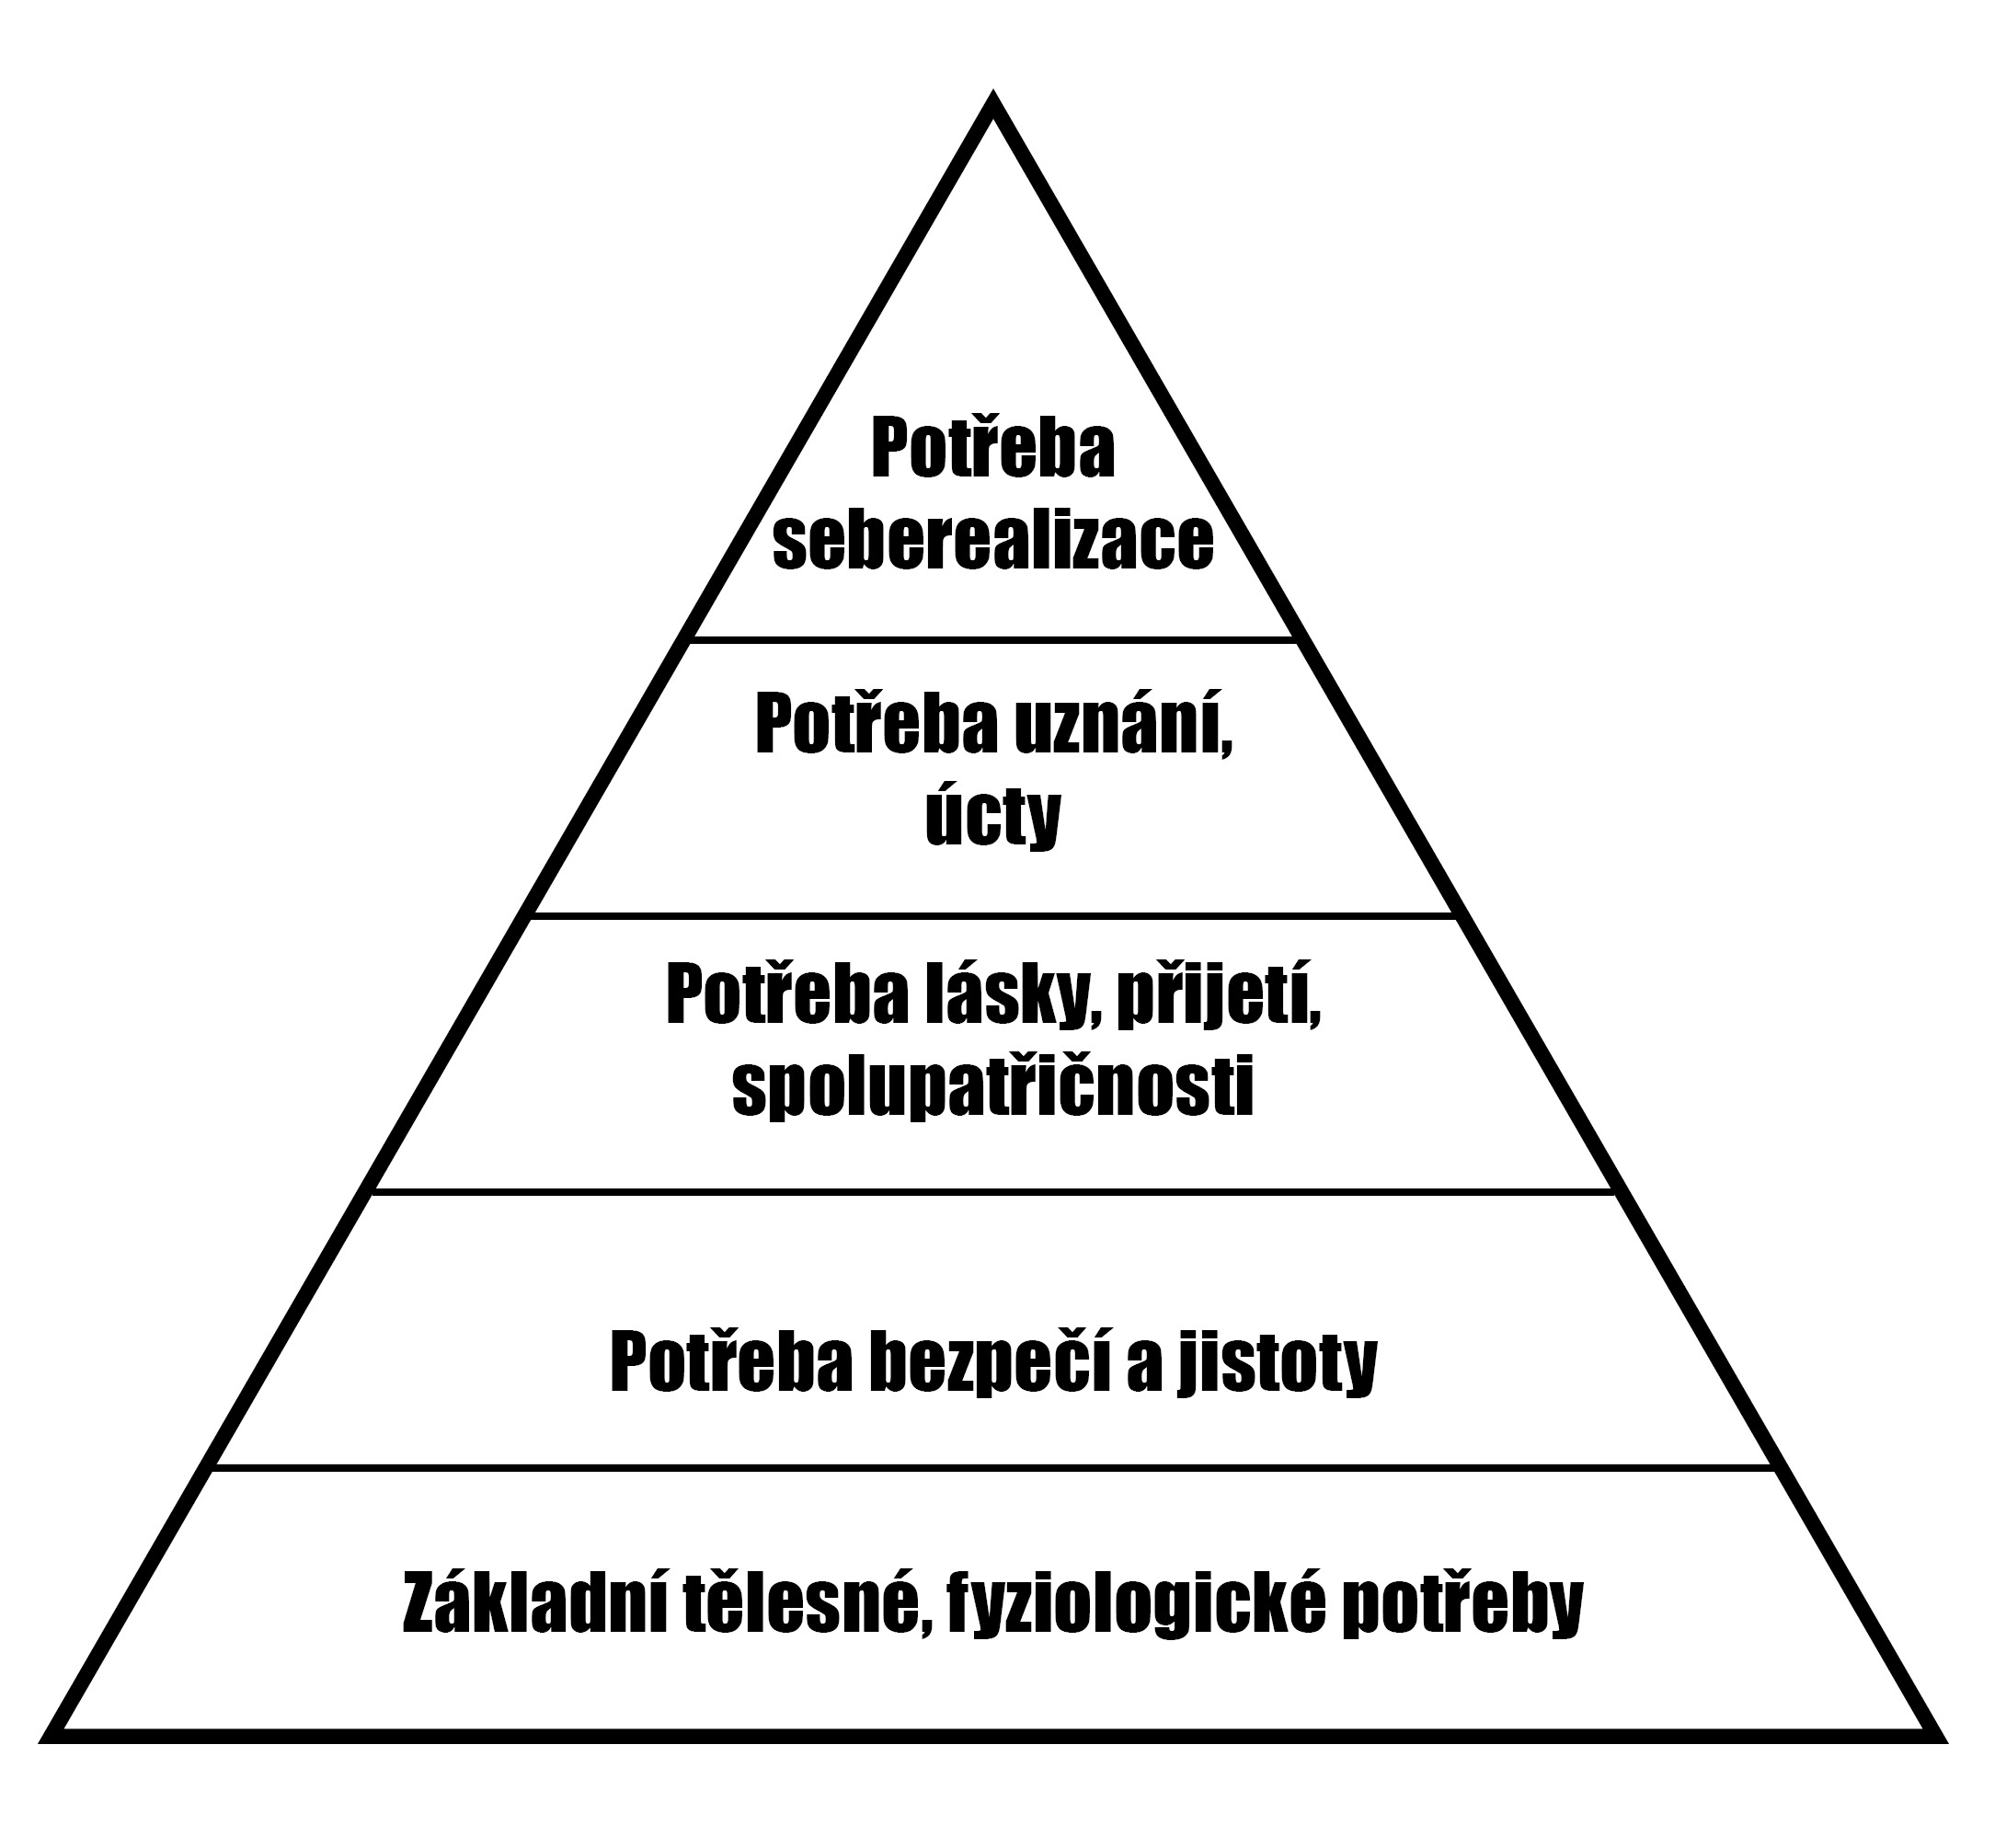
\includegraphics[width=0.8\textwidth]{\FIGDIR/maslow}
    \caption{Maslowova hierarchie potřeb\cite{wiki_potreby}}
    \label{fig:maslow}
\end{figure}

\begin{enumerate}
    \item \textbf{Fyziologické potřeby}: základní potřeby pro přežití, jako je potrava, voda, teplo a spánek
    \item \textbf{Potřeby bezpečí}: potřeby, které se týkají bezpečnosti a zabezpečení
    \item \textbf{Sociální potřeby}: potřeby, které se týkají příslušnosti, lásky a přátelství
    \item \textbf{Potřeby uznání}: potřeby, které se týkají úcty a sebeúcty
    \item \textbf{Potřeby seberealizace}: potřeby, které se týkají osobního růstu a rozvoje
\end{enumerate}

Jak to tedy ale souvisí s návrhem \ac{ui} a zejména s návrhem aplikace pro prodej vstupenek?

\textbf{Maslowova hierarchie potřeb} může být aplikována na návrh \ac{ui} tak, že každá úroveň hierarchie představuje jeden základní aspekt návrhu \ac{ui}.

V roce 2010 navrhl Steven Bradley v článku \textit{Designing For A Hierarchy Of Needs} podobnou hierarchii specificky pro design, se pěti odpovídajícími úrovněmi znázorněnými na obrázku~\ref{fig:design-hierarchy-of-needs}.\cite{bradley_hierarchy_of_needs}

\begin{figure}[H]
    \centering
    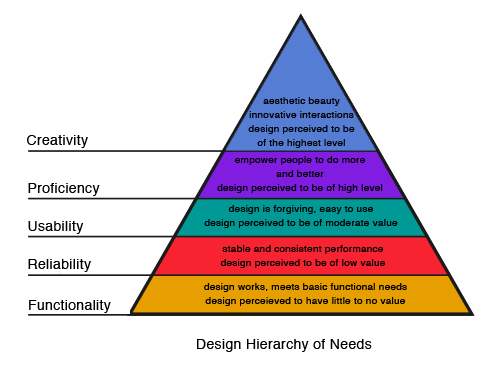
\includegraphics[width=0.8\textwidth]{\FIGDIR/design-hierarchy-of-needs}
    \caption{Hierarchie potřeb v návrhu \ac{ui} dle Stevena Bradleyho\cite{bradley_hierarchy_of_needs}}
    \label{fig:design-hierarchy-of-needs}
\end{figure}

\textbf{Funkčnost}: Na základě pyramidy jsou základní fyziologické potřeby.
V kontextu návrhu \ac{ui} to znamená základní funkčnost.
Aplikace musí fungovat tak, jak se očekává, aby si uživatelé mohli vybrat sedadlo, přidat vstupenku do košíku a dokončit proces objednávky bez jakýchkoli problémů.
Základní funkčnost musí být spolehlivá a robustní.

\textbf{Spolehlivost}: Další úroveň pyramidy je bezpečnost, která se v návrhu \ac{ui} týká spolehlivosti.
Rozhraní by mělo být navrženo tak, aby se uživatelé cítili bezpečně a sebevědomě při interakci s ním.
Poskytování jasných pokynů, okamžité zpětné vazby a potvrzení o úspěšných akcích (například přidání vstupenky do košíku) přispívá k pocitu bezpečí a použitelnosti.

\textbf{Použitelnost}: Střední část pyramidy pokrývá sociální potřeby, které se v \ac{ui} termínech rovnají uživatelské spokojenosti.
Esteticky příjemné rozhraní, personalizovaný uživatelský zážitek a interaktivní prvky (jako interaktivní plán sedadel) mohou významně zvýšit uživatelskou spokojenost.

\textbf{Odbornost}: Potřeby sebeúcty zahrnují touhu po uznání a respektu.
V kontextu aplikace pro prodej vstupenek by to mohlo znamenat přidání funkcí, které překračují očekávání uživatelů a zpříjemňují jim zážitek.
Může se jednat o něco tak jednoduchého, jako je blahopřání po úspěšném nákupu, nebo vizuální animace při výběru sedadla.

\textbf{Kreativita}: Na vrcholu pyramidy se nachází seberealizace, která se týká realizace osobního potenciálu a hledání osobního růstu a vrcholných zážitků.
Uživatelské rozhraní by mohlo přispět k této potřebě tím, že uživatelům umožní kreativně řešit problémy a dosáhnout svých cílů.
Například nabízení návrhů na nejlepší dostupná sedadla nebo podobných akcí může uživatele posílit a zlepšit jejich zážitek.

Použití Maslowovy hierarchie pro návrh \ac{ui} aplikace pro prodej vstupenek může pomoci zajistit, aby návrh splňoval potřeby uživatelů na různých úrovních.
Z počátku je nutné zajistit základní funkčnosti a spolehlivost, aby uživatelé mohli využívat aplikaci bez jakýchkoli problémů.
Dále je nutné zaměřit se na použitelnost, aby byl proces výběru sedadla a nákupu vstupenky co nejvíce zjednodušen.
Při postupu v hierarchii se budou zkoumat různé metody, jak zvýšit uživatelskou spokojenost a zlepšit jejich zážitek.
Cílem na vrcholu tohoto procesu je navrhnout rozhraní, které vyvažuje praktičnost a uživatelskou přívětivost, zatímco zároveň zajišťuje vizuální přitažlivost a emoční zapojení.
To povede k přínosnějšímu, uspokojivějšímu a úspěšnějšímu uživatelskému zážitku.

Další sekce se bude zabývat nástroji dostupnými pro návrh \ac{ui} a o důvodech pro výběr konkrétního nástroje pro tento projekt.

%%% TODO: Sekce - Nástroje pro návrh
%%% --------------------------------------------------------------
\section{Nástroje pro návrh}
\label{sec:navrh-ui-nastroje}
V oblasti návrhu uživatelského rozhraní má návrhář k dispozici širokou škálu nástrojů.
Tyto nástroje usnadňují nízkoúrovňové i vysokoúrovňové prototypování, přičemž každý z nich představuje jedinečnou sadu vlastností přispívajících k tvorbě, spolupráci a testování návrhů.
Tato sekce stručně popisuje tři nejčastěji používané nástroje pro návrh uživatelského rozhraní, a to Figma, Adobe XD a Sketch.

%%% TODO: Podsekce - Figma
%%% --------------------------------------------------------------
\subsection{Figma}
\label{subsec:navrh-ui-nastroje-figma}
Figma je nástroj pro návrh uživatelského rozhraní, který funguje v prohlížeči a je založen na cloudových technologiích.
Jeho hlavními výhodami jsou platformní nezávislost a snadná spolupráce.
Figma je také vybavena sadou funkcí, které usnadňují návrh uživatelského rozhraní, jako je vektorové kreslení, prototypování a předávání vývojářům.
\cite{figma}

\begin{figure}[H]
    \centering
    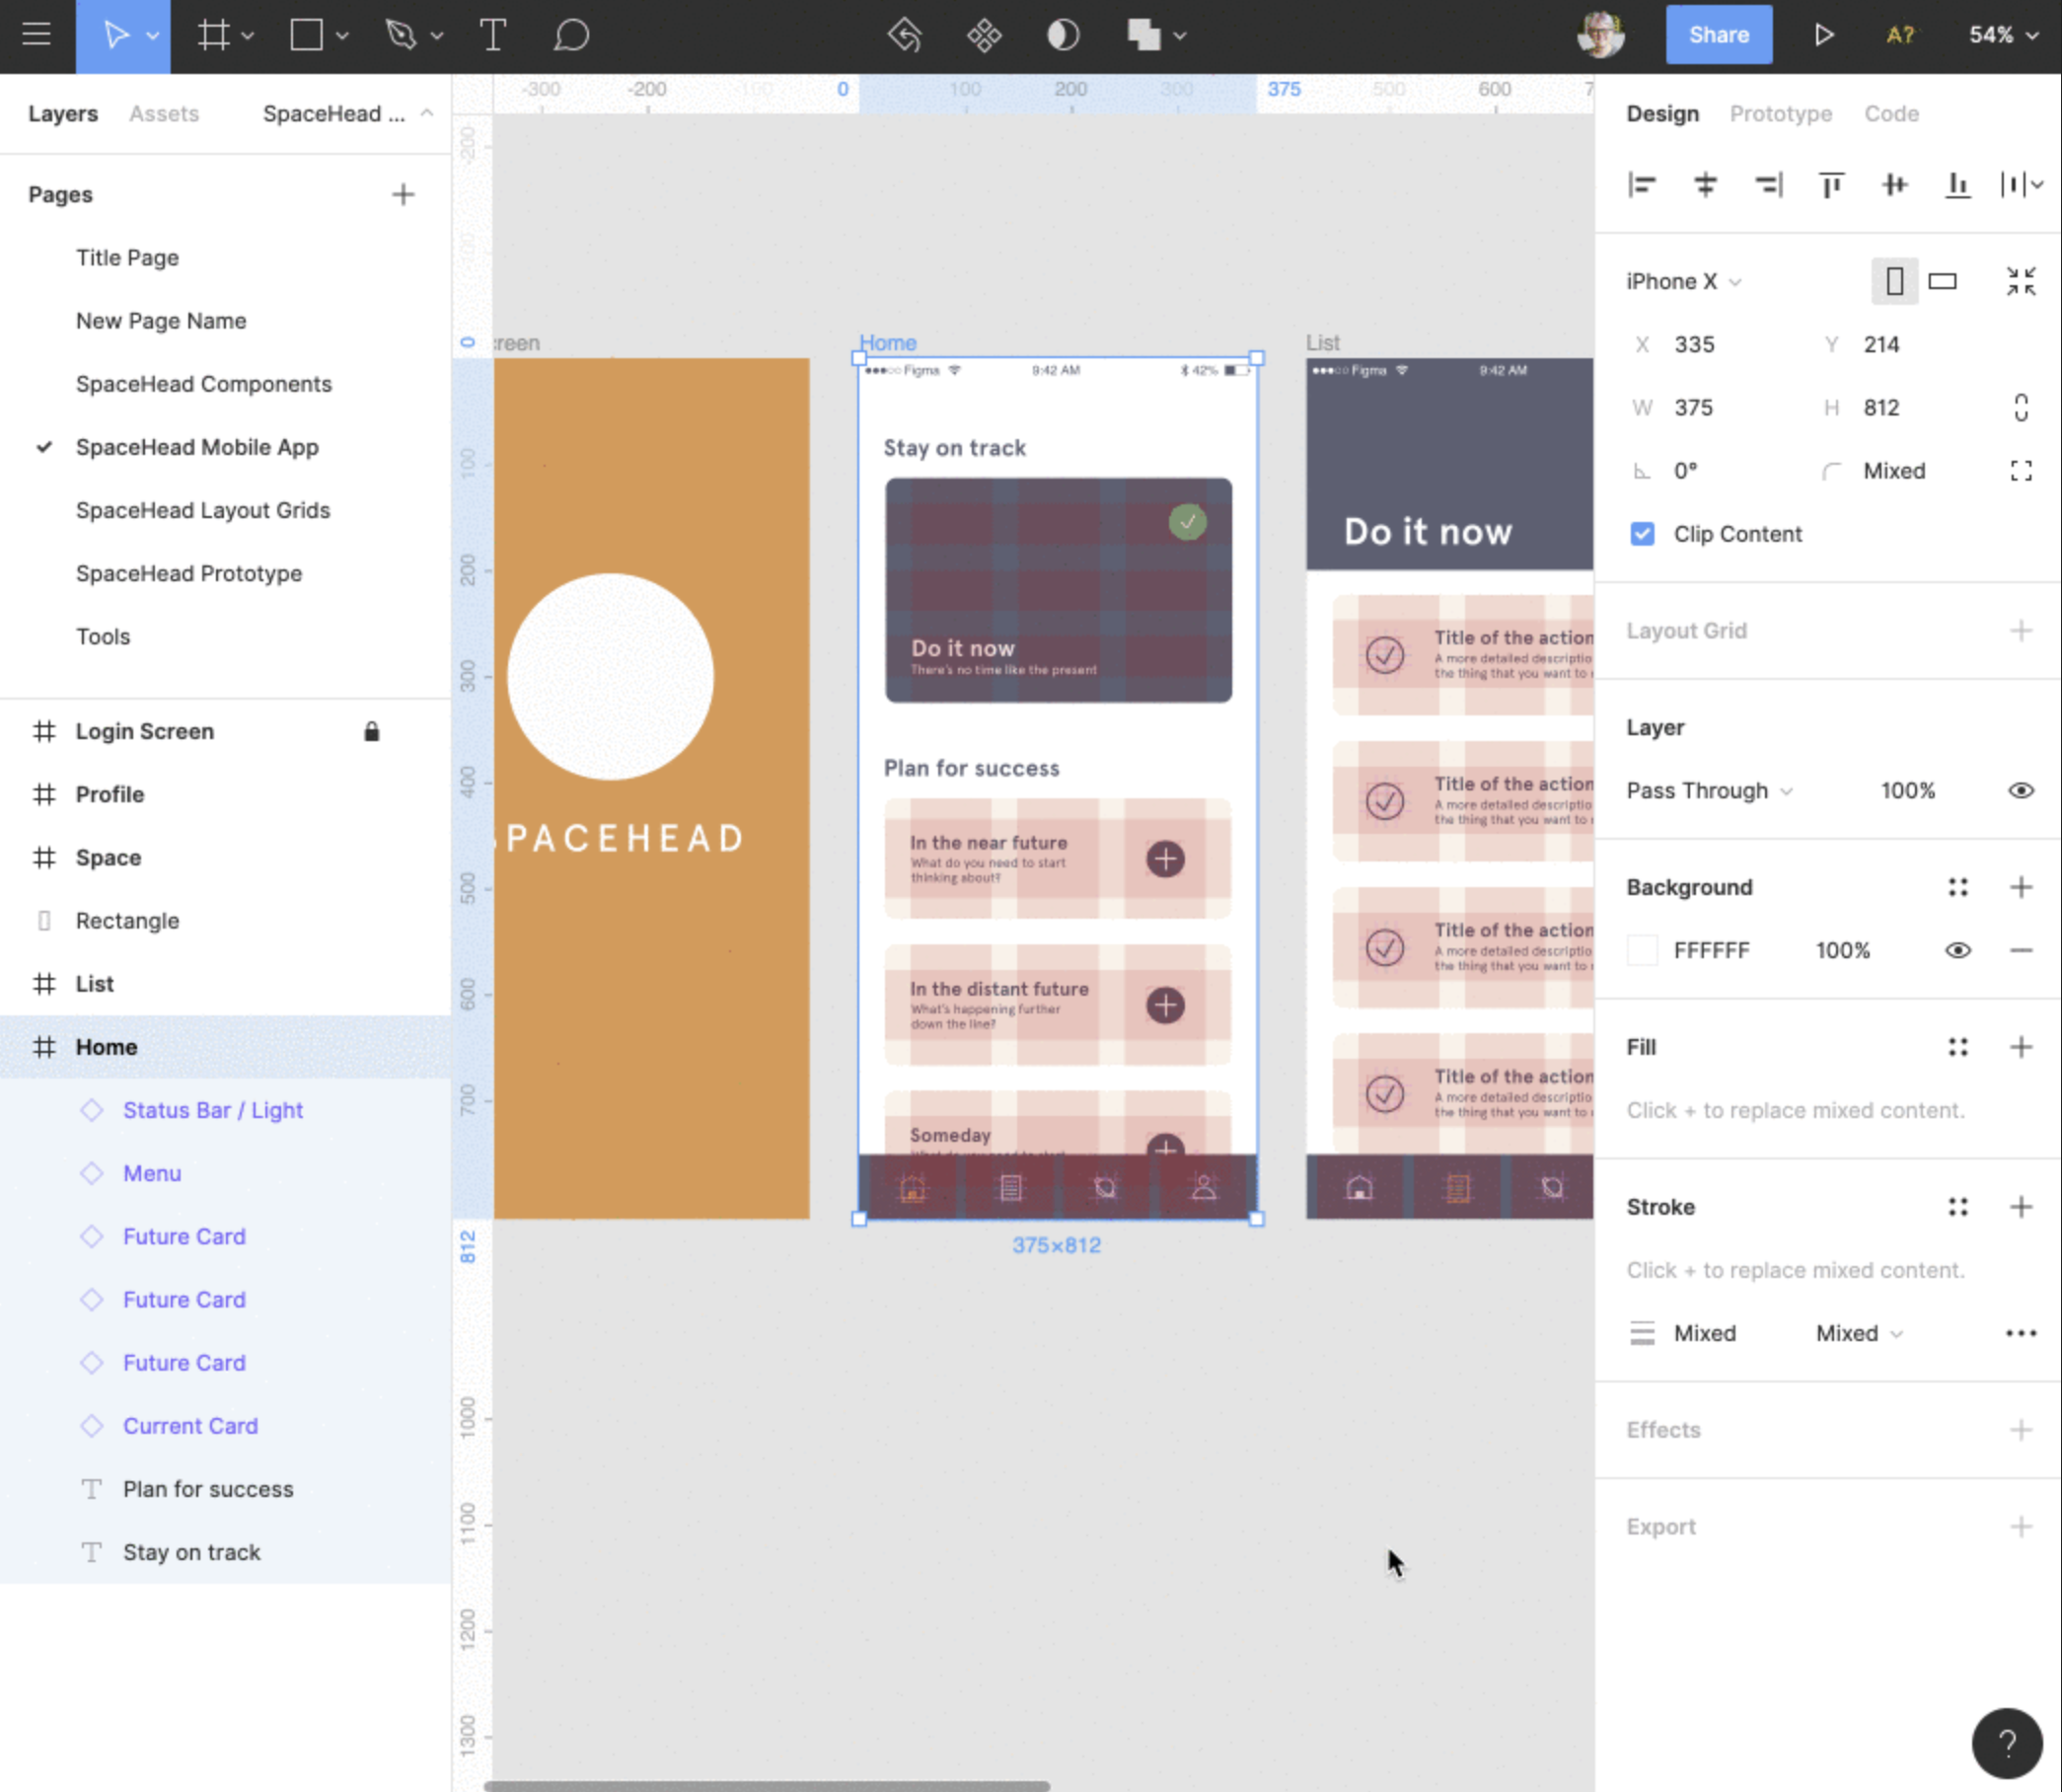
\includegraphics[width=0.8\textwidth]{\FIGDIR/figma}
    \caption{Ukázka nástroje Figma\cite{figma}}
    \label{fig:figma}
\end{figure}

%%% TODO: Podsekce - Adobe XD
%%% --------------------------------------------------------------
\subsection{Adobe XD}
\label{subsec:navrh-ui-nastroje-adobe-xd}
Adobe XD je nástroj od společnosti Adobe pro návrh uživatelského rozhraní, který funguje na platformách Windows i MacOS.
Jeho hlavními výhodami jsou jednoduché uživatelské rozhraní, prototypování a snadná integrace s ostatními produkty Adobe Suite.
\cite{adobe-xd}

\begin{figure}[H]
    \centering
    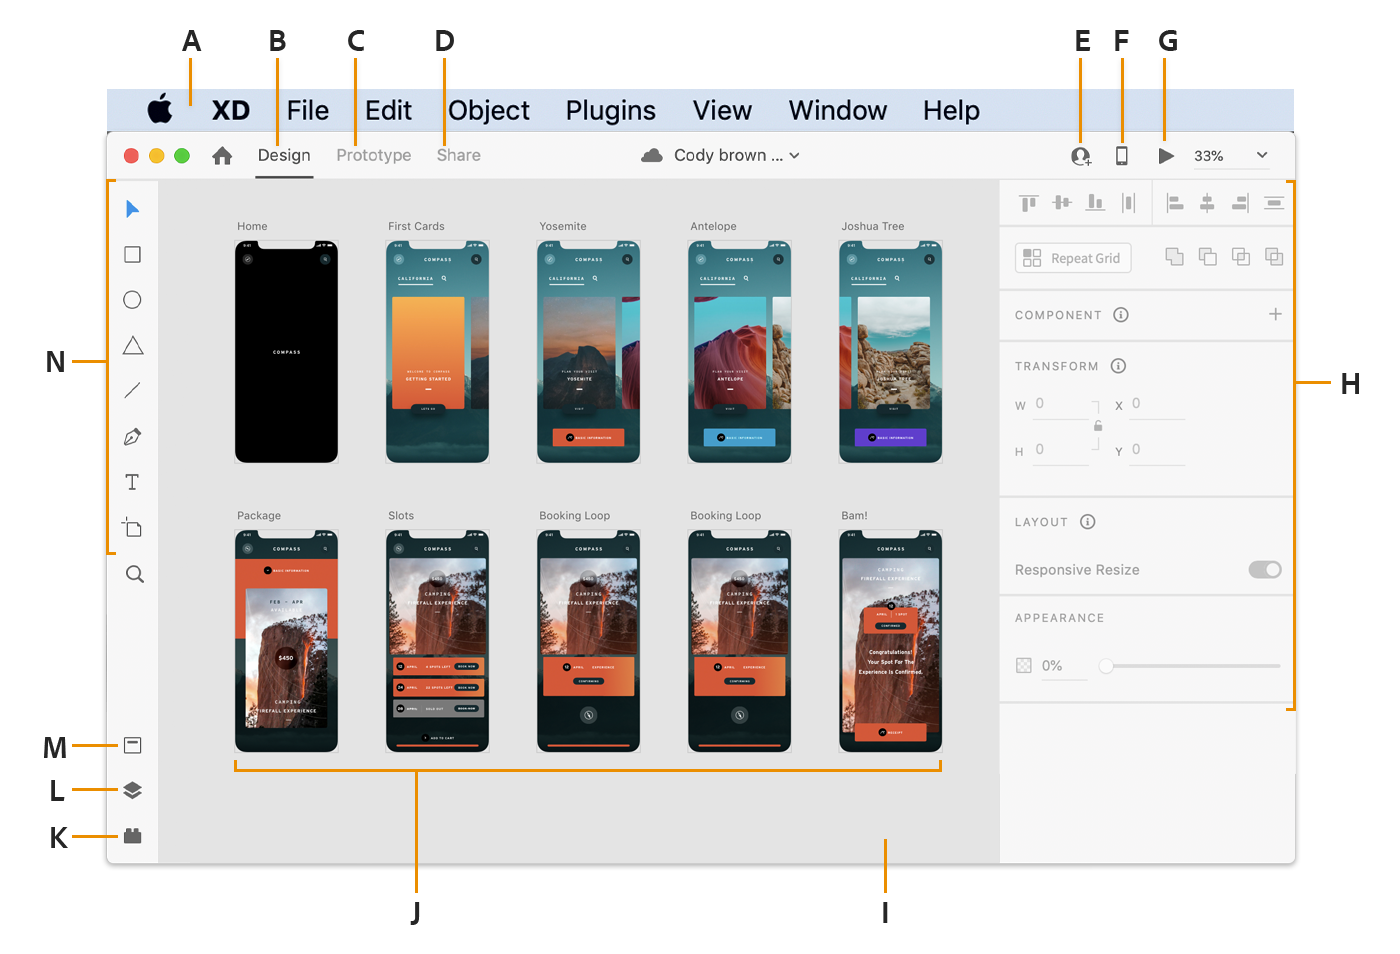
\includegraphics[width=0.8\textwidth]{\FIGDIR/adobe-xd}
    \caption{Ukázka nástroje Adobe XD\cite{adobe-xd}}
    \label{fig:adobe-xd}
\end{figure}

%%% TODO: Podsekce - Sketch
%%% --------------------------------------------------------------
\subsection{Sketch}
\label{subsec:navrh-ui-nastroje-sketch}
Sketch je nástroj pro návrh uživatelského rozhraní, který funguje výhradně na platformě MacOS.
Je to vektorový nástroj, který je chválen pro svou jednoduchost a rychlost.
Je užitečný při tvorbě rozhraní, webových stránek a ikon, i když absence vestavěných prototypovacích schopností může být pro některé návrháře omezujícím faktorem.
\cite{sketch}

\begin{figure}[H]
    \centering
    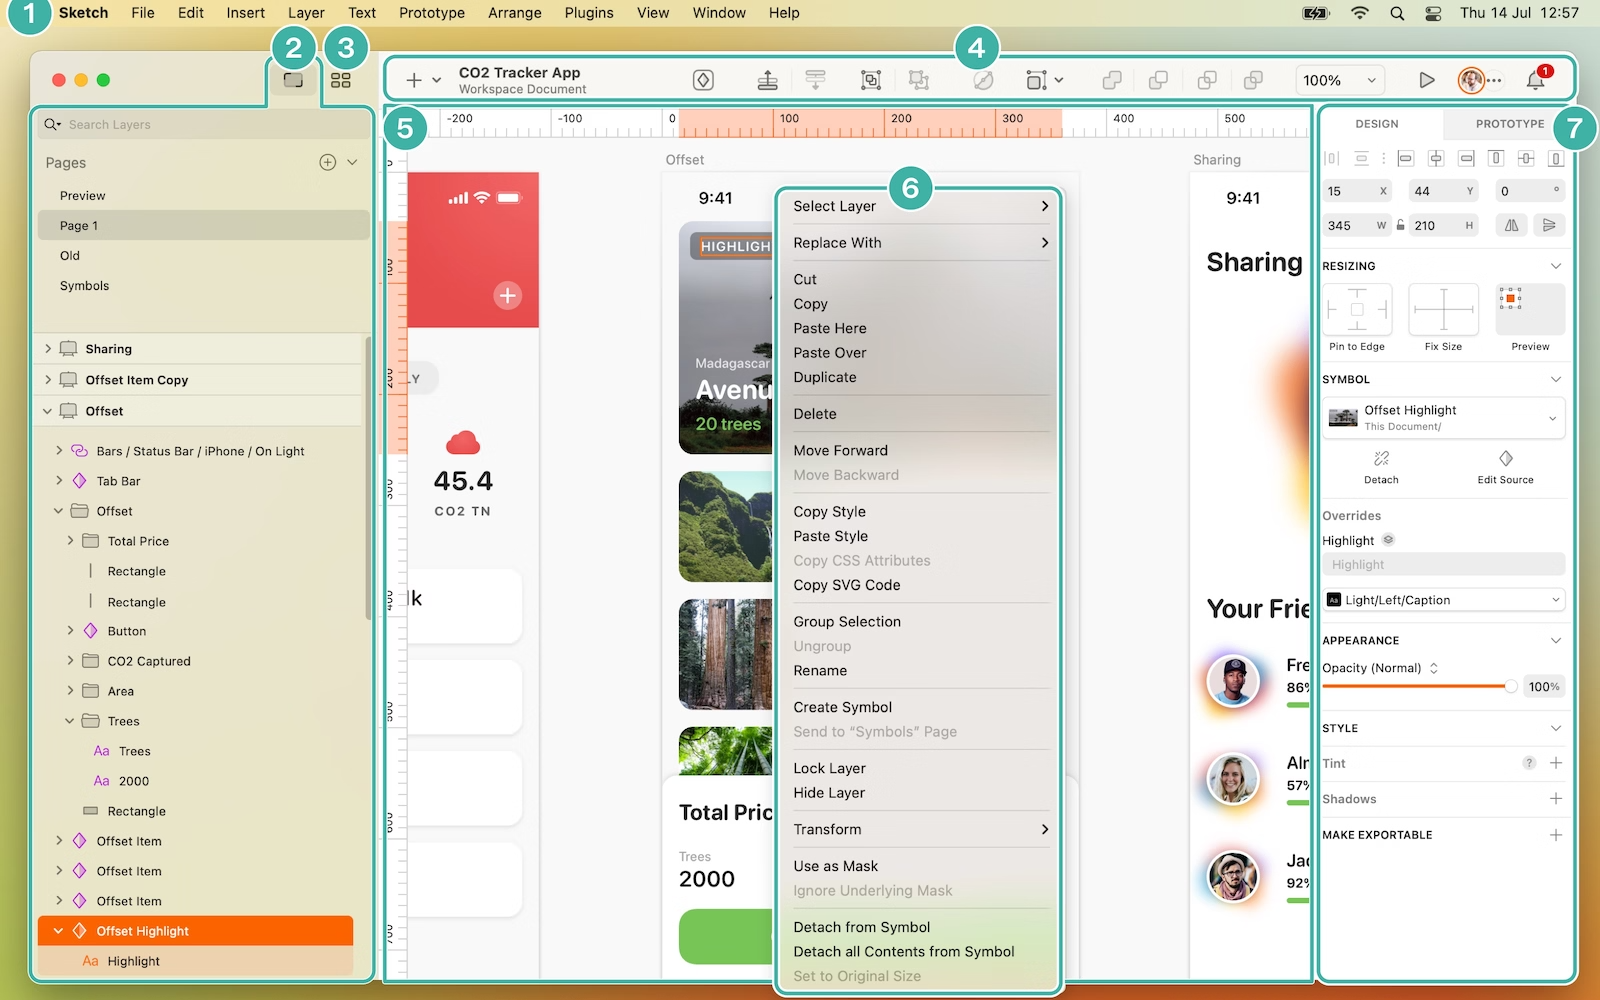
\includegraphics[width=0.8\textwidth]{\FIGDIR/sketch}
    \caption{Ukázka nástroje Sketch\cite{sketch}}
    \label{fig:sketch}
\end{figure}

%%% TODO: Podsekce - Výběr nástroje
%%% --------------------------------------------------------------
\subsection{Výběr nástroje}
\label{subsec:navrh-ui-nastroje-vyber}
Po podrobném zhodnocení byl pro návrh uživatelského rozhraní vyvíjené aplikace na prodej vstupenek s rezervací míst vybrán nástroj \textbf{Figma} z několika důvodů:

\textbf{Cloudově založený}: Figma umožňuje snadný přístup k návrhu z jakéhokoli zařízení, čímž odpadá nutnost instalace jakéhokoliv softwaru.
Nezáleží tedy ani na operačním systému, postačí pouze webový prohlížeč a připojení k internetu.

\textbf{Spolupráce v reálném čase}: I když se jedná o samostatný projekt, funkce spolupráce v reálném čase se ukazuje jako výhodná při poptávání zpětné vazby od možných budoucích zákazníků nebo konzultanta, čímž se zefektivňuje proces návrhu.

\textbf{Prototypování}: Rozsáhlé prototypovací schopnosti Figma usnadňují tvorbu interaktivních prototypů s vysokou kvalitou a důvěryhodností.

\textbf{Bezplatný}: Figma nabízí bezplatný plán, který je dostatečný pro většinu projektů.
Jedná se tedy o velmi výhodné řešení pro projekt, který není komerční či pro začínající návrháře.

\textbf{Vlastní zkušenost}: Osobně jsem měl možnost pracovat se všemi třemi nástroji a Figma se ukázala jako nejvhodnější pro tento projekt.
Zejména z důvodu jednoduchého uživatelského rozhraní, lehkosti použití a rychlosti prototypování.

%%% Sekce - Uživatelské příběhy
%%% --------------------------------------------------------------
\section{Uživatelské příběhy}
\label{sec:navrh-ui-uzivatelske-pribehy}
Při navrhování uživatelského rozhraní (\ac{ui}) nejde pouze o estetiku nebo funkčnost; vyžaduje to pochopení potřeb a očekávání uživatele.
Zahrnuje vytváření cesty, která uživatele bezproblémově provede aplikací a zároveň zajistí, aby mohli své úkoly vykonávat efektivně a s potěšením.
Technika, která se často používá v návrhu \ac{ui}/\ac{ux} k dosažení tohoto cíle, se nazývá \textit{User Stories} (uživatelské příběhy).
Uživatelské příběhy slouží jako nástroj, který pomáhá udržovat návrh zaměřený na uživatele a zajišťuje, že konečný produkt efektivně splňuje jeho potřeby.

Uživatelské příběhy, z anglického \foreign{User Stories}, jsou stručné, přímočaré popisy funkce nebo funkcionality, vyprávěné z pohledu uživatele.
Tyto příběhy kladou důraz na to, čeho uživatelé chtějí dosáhnout, podporují empatii a podporují návrhový proces, který se zaměřuje na uživatele.
Porozumění roli uživatelských příběhů při návrhu \ac{ui} webového řešení pro prodej vstupenek je klíčové pro efektivní splnění potřeb koncových uživatelů.

%%% TODO: Podsekce - Co jsou User Stories
%%% --------------------------------------------------------------
\subsection{Co jsou uživatelské příbehy}
\label{subsec:navrh-ui-uzivatelske-pribehy-co-jsou}

Uživatelské příběhy jsou součástí agilních vývojových praktik, široce používaných v návrhu \ac{ui}/\ac{ux} k zachycení zjednodušených popisů potenciálních funkcí aplikace z pohledu koncových uživatelů.
Slouží jako rychlý a jednoduchý způsob, jak popsat uživatele, co chtějí a proč to chtějí.
Každá \foreign{User Story} následuje strukturovaný formát:

\begin{gray-box}{Formát uživatelského příběhu}
    ``\textbf{Jako} [\textit{typ uživatele}] \textbf{chci} [\textit{vykonat nějakou akci}], \textbf{abych} [\textit{dosáhl nějakého cíle}].``
\end{gray-box}

V tomto formátu:
\begin{itemize}
    \item \textbf{Typ uživatele} pomáhá definovat roli uživatele, který bude používat danou funkcionalitu.
    \item \textbf{Vykonat nějakou akci} umožňuje zjistit, co chce uživatel pomocí dané funkcionality udělat nebo čeho chce dosáhnout.
    \item \textbf{Dosáhl nějakého cíle} vysvětluje základní motivaci nebo hodnotu, kterou uživatel získá provedením akce.
\end{itemize}

Tento formát je velmi užitečný při vytváření uživatelských příběhů, jelikož pomáhá udržovat stručnost, jednoznačnost a zároveň poskytuje dostatek informací, aby bylo možné pochopit, co uživatel chce a proč to chce.

Uživatelské příběhy hrají také klíčovou roli při definování akceptačních kritérií, která dále podrobně popisují, jak by měla určitá funkce fungovat z pohledu uživatele.
To pomáhá stanovit jasnou představu o účelu a očekávaném chování funkce, čímž usměrňuje její vývoj a testování.

V kontextu navrhovaného uživatelského rozhraní pro webové řešení prodeje vstupenek mohou tyto uživatelské příběhy pomoci přesně určit funkcionality, které jsou pro uživatele nejdůležitější.
Pomáhají porozumět potencionálním uživatelům –~návštěvníkům událostí, jejich potřebám (jako jsou např.\ prohlížení místa konání, výběr sedadel), jejich akce (přidání vstupenek do košíku, přechod k zaplacení) a jejich motivaci (užít si bezproblémový nákup vstupenek).

Následující sekce se zabývá tím, jak lze uživatelské příběhy konkrétně použít k navrhování uživatelského rozhraní.

%%% TODO: Podsekce - Psaní efektivních uživatelských příběhů
%%% --------------------------------------------------------------
\subsection{Psaní efektivních uživatelských příběhů}
\label{subsec:navrh-ui-uzivatelske-pribehy-psani-efektivnich}

Při psaní efektivních uživatelských příběhů pro platformu prodeje vstupenek je klíčové porozumět perspektivě koncového uživatele.
Tento proces vyžaduje identifikaci potřeb, motivací a požadovaných výsledků uživatele při používání platformy.
Některé očekávané úkoly pro platformu prodeje vstupenek mohou zahrnovat prohlížení události, výběr sedadla a dokončení nákupu vstupenky.

První krok je identifikace a pochopení různých ``personas`` nebo typů uživatelů, kteří budou pravděpodobně s platformou interagovat.
Pro platformu prodeje vstupenek je primárním uživatelem obvykle někdo, kdo má zájem o nákup vstupenek na události.
Sekundární uživatelé, jako jsou organizátoři událostí nebo manažeři prostorů, však mohou také s platformou interagovat s odlišnými požadavky na funkcionalitu.

Dalším krokem je zjištění, co uživatelé chtějí dosáhnout.
To může zahrnovat jednoduché úkoly, jako je ``prohlížení nadcházejících událostí``, nebo složitější úkoly, jako je ``rezervace místa na konkrétní událost``.
Každý uživatelský příběh by měl zůstat stručný a zaměřený na jednu akci.

Posledním krokem je definování ``hodnoty`` nebo ``výhody``, kterou uživatel získá provedením dané akce, což je známé jako jeho motivace.
Tento krok je klíčový, protože pomáhá při prioritizaci funkcí na základě hodnoty, kterou poskytují uživateli.

Při tvoření těchto uživatelských příběhů je užitečné dodržovat princip \foreign{INVEST} (\foreign{Independent}, \foreign{Negotiable}, \foreign{Valuable}, \foreign{Estimable}, \foreign{Small}, \foreign{Testable}).
Tento princip zajišťuje, že každý uživatelský příběh je dobře definován a má potřebné charakteristiky pro efektivní implementaci v procesu vývoje.

Příkladem uživatelského příběhu pro platformu prodeje vstupenek může být:

\begin{gray-box}{Ukázka uživatelského příběhu}
    \textit{``Jako zákazník si chci být schopen vybrat konkrétní sedadlo, abych se mohl akce zúčastnit.``}
\end{gray-box}

Tento uživatelský příběh je nezávislý na ostatních uživatelských příbězích, je jednoduchý a snadno pochopitelný, poskytuje hodnotu uživateli a je snadno testovatelný.
Při dodržení tohoto principu mohou uživatelské příběhy poskytnout cenný náhled do toho, jak by měla platforma prodeje vstupenek fungovat z pohledu uživatele.

%%% TODO: Podsekce - Uživatelské příběhy aplikace
%%% --------------------------------------------------------------
\subsection{Uživatelské příběhy aplikace}
\label{subsec:navrh-ui-uzivatelske-pribehy-aplikace}
Na základě pochopení získaného v předchozích sekcích se lze nyní zaměřit na konstrukci konkrétních uživatelských příběhů pro implementované webové řešení prodeje vstupenek s rezervací míst.
Nejprve je však nutné definovat hlavní uživatelský typ, který bude tuto aplikaci používat.
V základu lze říci, že hlavní rolí uživatele je potencionální zákazník, který má zájem o nákup vstupenky na konkrétní událost.
Pro další účely bude ale použito pouze záměrné označení ``zákazník``.
Každý příběh bude představen ve stanoveném formátu.
Dále budou sepsána určitá kritéria přijatelnosti, dle kterých bude jednoduše zhodnotitelné splnění příběhu.
Na závěr bude diskutováno o tom, jak daný příběh ovlivňuje návrh uživatelského rozhraní.

\begin{gray-box}{Uživatelský příběh 1 – Vizualizace místa konání}
    \textit{``Jako zákazník, chci vidět, jak vypadá místo konání, abych si mohl vybrat místo, které mi bude vyhovovat.``}
\end{gray-box}

Tento uživatelský příběh zdůrazňuje důležitost jasné a intuitivní vizualizace místa konání.
Mapa musí poskytovat přesnou reprezentaci uspořádání sedadel a nabízet dostatek detailů, aby uživatelé mohli snadno vybrat místo, které jim vyhovuje.
Pro tento příběh lze kritéria přijatelnosti definovat jako:
\begin{enumerate}
    \item Mapa místa konání je dobře viditelná
    \item Mapa místa konání přesně reprezentuje uspořádání sedadel
    \item Sedadla na mapě jsou jasně označena a snadno rozpoznatelná
\end{enumerate}

\begin{gray-box}{Uživatelský příběh 2 – Výběr sedadla}
    \textit{``Jako zákazník, si chci označit či odznačit konkrétní sedadla, abych si mohl vybrat místa, která mi budou vyhovovat.``}
\end{gray-box}

Flexibilní výběr sedadla je klíčovým prvkem prodeje vstupenek.
Uživatelé by měli mít možnost vybrat si konkrétní sedadlo, které jim vyhovuje, a měli by mít možnost si vybrat více sedadel, pokud si přejí sedět s přáteli nebo rodinou.
Uživatelské rozhraní by tedy mělo uživatelům umožnit snadno vybrat a zrušit výběr sedadel, aby mohli vyzkoušet různé možnosti výběru, které jsou k dispozici.
Pro tento příběh jsou kritéria přijatelnosti následující:
\begin{enumerate}
    \item Uživatelé mohou kliknutím vybrat konkrétní sedadlo
    \item Uživatelé mohou vybrat více sedadel
    \item Zvolená sedadla jsou jasně označena
    \item Uživatelé mohou kliknutím zrušit výběr sedadla
\end{enumerate}

\begin{gray-box}{Uživatelský příběh 3 – Nákupní košík}
    \textit{``Jako zákazník, chci mít jasný přehled o přidaných vstupenkách do nákupního košíku, abych měl přehled o svém nákupu.``}
\end{gray-box}

Tento uživatelský příběh například zdůrazňuje důležitost uživatelského rozhraní nákupního košíku se vstupenkami.
Uživatelé by měli mít možnost snadno zobrazit, jaké vstupenky mají v nákupním košíku, a měli by mít možnost snadno upravovat jeho obsah.
To vyžaduje jednoduché a přístupné uživatelské rozhraní spravující funkci nákupního košíku.
Pro přijetí tohoto příběhu jsou adekvátní kritéria přijatelnosti:
\begin{enumerate}
    \item Uživatel může snadno zobrazit aktuálně přidané vstupenky v nákupním košíku
    \item Uživatel může upravovat přidané vstupenky v košíku
    \item Uživatel může vstupenky z košíku odebrat
    \item Uživatel může zobrazit celkovou cenu nákupu
\end{enumerate}

\begin{gray-box}{Uživatelský příběh 4 – Vyřízení objednávky}
    \textit{``Jako zákazník, chci jasný a jednoduchý proces vyřízení objednávky, abych mohl svůj nákup vstupenek sebejistě dokončit.``}
\end{gray-box}

Poslední zmíněný uživatelský příběh se zaměřuje na proces vyřízení objednávky.
Zdůrazňuje potřebu jednoduchého a intuitivního uživatelského rozhraní, které umožní uživatelům snadno dokončit svůj nákup vstupenek.
Uživatelské rozhraní dokončení objednávky by tedy mělo minimalizovat komplexitu a zmatečnost, čímž zajistí uživatelům důvěru při dokončování své objednávky.
Pro tento příběh sestrojit kritéria přijatelnosti následovně:
\begin{enumerate}
    \item Proces dokončení objednávky je jednoduchý a intuitivní
    \item Objednávku lze dokončit v několika málo krocích
    \item Uživatel obdrží potvrzení o dokončení objednávky
\end{enumerate}

Z důvodu zachování přehlednosti a jednoduchosti, ačkoliv by mohlo být vytvořeno více uživatelských příběhů, budou v této práci použity pouze tyto čtyři hlavní uživatelské příběhy.
Tyto příběhy, budou v následující kapitole použity jako základní stavební kameny pro návrh uživatelského rozhraní vyvíjené webové aplikace.


%%% Sekce - Návrh UI mapy
%%% --------------------------------------------------------------
\section{Návrh UI mapy}
\label{sec:navrh-ui-mapa}
TODO: navrh rozhraní mapy, sedadel, hlavní komponenta
